\section{Method}

\subsection{Network architecture}


\begin{figure}
\centering

% TODO should mention sizes! Maybe represent decoder output differently.

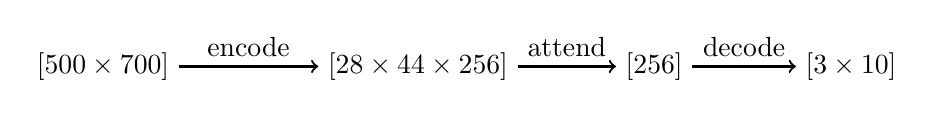
\begin{tikzpicture}
% 900, 1500, 1
% 28, 44, 256
% 1, 1, 256
% 3, 10

    \node (input) at (0,0) {$[500 \times 700]$};
    \node (encoded) at (4, 0) {$[28 \times 44 \times 256]$};
    \node (attended) at (7, 0) {$[256]$};
    \node (decoded) at (9.5, 0) {$[3 \times 10]$};

%   \pic [fill=cyan, draw=blue] at (-1,0) {annotated cuboid={width=1, height=900, depth=1500}};
%   \pic [fill=cyan, draw=blue] at (4,-0.5) {annotated cuboid={width=256, height=28, depth=44}};
%   \pic [fill=cyan, draw=blue] at (7,-0.5) {annotated cuboid={width=256, height=1, depth=1}};
%   \pic [fill=cyan, draw=blue] at (9,1.5) {annotated cuboid={width=1, height=10, depth=3}};

  \draw [->,thick] (input) -- node [above] {encode} (encoded);
  \draw [->,thick] (encoded) -- node [above] {attend} (attended);
  \draw [->,thick] (attended) -- node [above] {decode} (decoded);

\end{tikzpicture}

\caption{Overview of how the data flows in the proposed network. First the encoder produces a matrix of feature vectors, each corresponding to a different but overlapping location in the input image. Secondly, the attention aggregates the feature vectors into a single feature vector. Lastly, the decoder produces three softmax outputs, one for each digit.}
\label{fig:sys_overview}
\end{figure}


We now describe the different parts of the proposed network. See figure \ref{fig:sys_overview} for an overview of how the different parts of the network interact.

\subsubsection{Experiments}
% TODO: write here or somewhere completely different?

\subsubsection{Encoder}

\begin{figure}
\centering

\begin{tikzpicture}
% (1, 900, 1500, 1)
% (1, 450, 750, 4)
% (1, 225, 375, 16)
% (1, 225, 375, 32)
% (1, 112, 187, 32)
% (1, 112, 187, 128)
% (1, 56, 93, 128)
% (1, 56, 89, 256)
% (1, 28, 44, 256)

%   \pic {annotated cuboid};
  \pic [fill=cyan, draw=blue] at (0,0) {annotated cuboid={width=32, height=900, depth=1500}};
  \pic [fill=cyan, draw=blue] at (0.5,0) {annotated cuboid={width=32, height=900, depth=1500}};

  \pic [fill=yellow, draw=white] at (1.5,-0.5) {annotated cuboid={width=32, height=450, depth=750}};
  \pic [fill=cyan, draw=blue] at (2.1,-0.5) {annotated cuboid={width=64, height=450, depth=750}};
  \pic [fill=cyan, draw=blue] at (2.7,-0.5) {annotated cuboid={width=64, height=450, depth=750}};

  \pic [fill=yellow, draw=white] at (3.5,-0.7) {annotated cuboid={width=64, height=225, depth=375}};
  \pic [fill=cyan, draw=blue] at (4.5,-0.7) {annotated cuboid={width=128, height=225, depth=375}};

  \pic [fill=yellow, draw=white] at (5.5,-0.7) {annotated cuboid={width=128, height=112, depth=187}};
  \pic [fill=cyan, draw=blue] at (6.5,-0.7) {annotated cuboid={width=128, height=112, depth=187}};

  \pic [fill=yellow, draw=white] at (7.5,-0.8) {annotated cuboid={width=128, height=56, depth=93}};
  \pic [fill=green, draw=blue] at (9,-0.8) {annotated cuboid={width=256, height=56, depth=89}};

  \pic [fill=yellow, draw=white] at (10.5,-0.8) {annotated cuboid={width=256, height=28, depth=44}};

%   \pic [fill=magenta, text=blue, draw=blue] at (5,0) {annotated cuboid={width=2, height=50, depth=30}};
%   \pic [fill=green, text=green!50!black, draw=green!25!black] at (5,-2) {annotated cuboid={width=6, height=20, depth=15, units=mm}};
%   \pic at (1,-3) {annotated cuboid={width=150, height=200, depth=250, scale=.01, units=m}};
%   \pic [fill=cyan, text=blue!75!cyan, draw=blue!75!cyan] at (-3,-2) {annotated cuboid={width=15, height=18, depth=13.5, units=}};
\end{tikzpicture}

\caption{Proposed architecture for the encoder. Convolutional layers are blue (3x3) and green (1x5) while max pool layers are yellow (2x2).
The number below each layer indicate the depth of the layer.}
\label{fig:encoder}
\end{figure}


For encoder, we use a CNN with 7 convolutional layers with additional pooling layers, see figure \ref{fig:encoder}.
% We experimented with several different variations in number of convolution layers, pooling layers and layer depths before choosing this model.
Two consecutive 3x3 convolutional layers is a refactoring of a single 5x5 layer as suggested by \cite{InceptionV3}. Thus, the first four convolutional layers correspond to two 5x5 convolutional layers with pooling, similar to the original single digit CNN classifier \cite{lecun_1989} but with greater depth.

The number of pooling layers, number of convolutional layers and depth per layer were determined experimentally. The final encoder design, as in figure \ref{fig:encoder}, is somewhat similar to the encoder used in \cite{FornesCnnCategorization} except that we use more aggressive pooling. This is necessary because in our work, we input images of entire pages while \cite{FornesCnnCategorization} classify word images which presumably are much smaller.

%The first four layers correspond closely to the original single digit classifier CNN \cite{lecun_1989} with the exception

% The number of layers and their depth was determined experimentally on the synthesized dataset using previous work as starting point \cite{FornesCnnCategorization}.

% TODO describe experiments.



\subsubsection{Attention model}

Another major difference between our work and \cite{FornesCnnCategorization} is that although we both use variable input size, they use \textbf{Spatial pyramid pooling} while we apply a soft attention model as presented in \cite{AttendAndTell}. Like we discussed previously in \ref{ssec:attention}, the encoder output can be seen as a list of feature vectors $\mathbf{a_i} \in \mathbb{R}^D$ which correspond to different but overlapping locations. The number of produced feature vectors depends on the size of the input image. We will see that this attention model aggregates all feature vectors $\mathbf{a_i}$ into a single fixed size vector $\mathbf{z} \in \mathbb{R}^D$.

The attention model consists of a multilayer perceptron which for each feature vector $\mathbf{a_i}$ computes a salience score $e_i$:

\[
e_i = f_\text{MLP}(\mathbf{a_i})
\]

Note that this MLP does not have access to any information about the corresponding location of $\mathbf{a_i}$, thus the network must learn to recognize important parts by looking at the encoded features alone instead of learning to always look at a certain position in the input image. This is especially important for population records where the relevant information can be in different locations depending on scribe and time period.

As discussed, we normalize the $e_i$ into $\alpha_i$ by computing the softmax. Then we use the attentions $\{\alpha_i\}$ as weights over the feature vectors:

\[
\mathbf{z} = \sum_{k=1}^L \alpha_i \mathbf{a_i}
\]

Note that the spatial information about where in the image $\mathbf{z}$ comes from is lost in this sum. So just like the attention MLP, the decoder also becomes invariant to the object's position in the input image.

\subsubsection{Decoder}

The decoder employs an MLP for classifying the aggregated feature vector $\mathbf{z}$ from the attention model.
If $\mathbf{z}$ had a variable length, then we would need a different number of weights in the MLP for each different input size. Since the attention model produces a fixed size output independent of input size we avoid the problem of variable number of parameters.

The proposed MLP consist of one fully connected layer of $1024$ neurons with dropout as well as three parallel readout layers, each with a size of $10$ neurons. The three separate outputs correspond to one digit each.


\subsection{Pre-training}
\subsection{Labeling}
\subsection{Training}
\subsection{Evaluation}


% TODO should technologies/implementation be described in a different section?
% Is it at all relevant to discuss about Tensorflow?
\subsection{Tensorflow}
% TODO Mention GPU acceleration here or in section about neural networks?

\subsection{Hardware}
% TODO Mention hardware and training time .
